\title{CS378 Architecture: \\ Cache Replacement Report}
\author{Rushi Shah}
\date{\today}

\documentclass[9pt]{article}
\usepackage{graphicx}
\usepackage{url}
\usepackage[margin=1.2in]{geometry}

\begin{document}

\maketitle

\section{Experiments}

	\subsection{Simulate OPT}

		Belady's algorithm was implemented to simulate the optimal solution. A trace file containing a sequence of memory addresses was used to predict the future. For each address, a queue was constructed that stores the ``timestamp'' when that address was referenced (where the timestamp is just the index of the reference in the trace file). When an address is referenced in the simulation, an element is popped off the queue for that address. On a cache miss, the implementation will peek at the head of the queue for the address in each way of the cache and identify the largest value (or infinity represented by an empty queue) which is then selected as the victim. This approach implements Belady's algorithm because it selects the way with the longest re-reference interval. 

	\subsection{Custom Design: Constant \& ``Round Robin''}

		As a naive baseline, two simple algorithms were implemented: the ``constant'' algorithm and the ``round-robin'' algorithm. The constant algorithm simply evicts the seventh way on every miss. Similarly, the round robin algorithm cycles through each of the $n$ ways in the cache by evicting way 0, then way 1, then way 2, then way 3, \ldots, then way $n$, then way 1, then way 2, \ldots.

	\subsection{Custom Design: ``Static Rereference Interval Prediction''}

		As a custom implementation, the static re-reference interval prediction algorithm was lifted from ``High Performance Cache Replacement Using Re-Reference Interval Prediction (RRIP)'' (\url{https://people.csail.mit.edu/emer/papers/2010.06.isca.rrip.pdf}). This approach maintains a map from a block addresses to an $M$ bit saturating counter that represents the rereference interval prediction for that address. Lower values for the saturating counter represent more immediate re-reference predictions, and values are inserted with a default value of $2^M - 2$. When an address hits in the cache, it is predicted to hit again soon, so its counter is decremented. To select a victim, the implementation will iterate through all the addresses in each way seeking an address that has a current prediction of $2^M - 1$, which will be ultimately selected as the victim. If all the current addresses are lower than that, they are all incremented and the search is repeated. Experiments were conducted with $M = 2$ and $M = 5$, and our experiments corroborated the paper's claim that $M = 2$ is sufficient. 
	

\section{Results}

	The included graphs summarize the results of the experiments. 

	All graphs measure misses per kilo-instructions (MPKI) which is a standard metric in the computer architecture literature (lower bars are better). The benchmarks are ordered from least to greatest MPKI in the optimal solution (which means the Average measurements are listed as the fifth set of bars in each chart). 

	The first graph only shows the performance of LRU (the baseline), SRRIP (with $M = 2$), and OPT (Belady's algorithm).

	The second graph shows the ``round robin'' algorithm compared to the constant replacement algorithm measured against the LRU baseline. 

	The third graph shows the same implementation of Static RRIP configured with two different parameter values ($M = 2$ and $M = 5$). 

	The fourth, and final, graph shows the performance of all the experiments aggregated into one graph. 

	Scroll to the bottom of the report to see the graphs.

\section{Conclusions}

	The SRRIP algorithm represents an improvement over the baseline of LRU, but still does not substantially close the significant gap between LRU and OPT. Thus, Figure 1 shows that although SRRIP is better than the naive solution, there is clearly room for improvement. 

	The round-robin algorithm shows slightly better performance than the constant algorithm, which makes sense because it utilizes more of the cache than the constant algorithm. The round-robin algorithm is appealing because it requires virtually no overhead. Perhaps surprisingly, both the constant and the round robin algorithms outperform LRU in the average case, despite requiring less overhead. These conclusions can be drawn most clearly from Figure 2. 

	SRRIP is configured with a parameter $M$ which represents the number of bits stored for the saturating counters. A lower $M$ is better in terms of overhead, but it was worth exploring if a larger $M$ could improve performance. As we can see in Figure 3, more than doubling the number of bits utilized for the saturating counters has an imperceptible impact on MPKI. This might be because the effect of the longer saturating time for the larger counters is overshadowed by the relative lengths of the rereference interval predictions (i.e. having a longer saturating counter doesn't reorder the interval predictions in relation to each other). This is good news because it corroborates the paper's claim that $M = 2$ is sufficient. 

	Finally, Figure 4 aggregates the results of all experiments into one chart for convenient comparisons on a shared scale. From this graph, we can see that ``round-robin'' is the unexpected star: it requires negligible overhead and yet achieves performance the closest to OPT in the average case. 
 
\pagebreak

\begin{figure}[t]
  \centering
  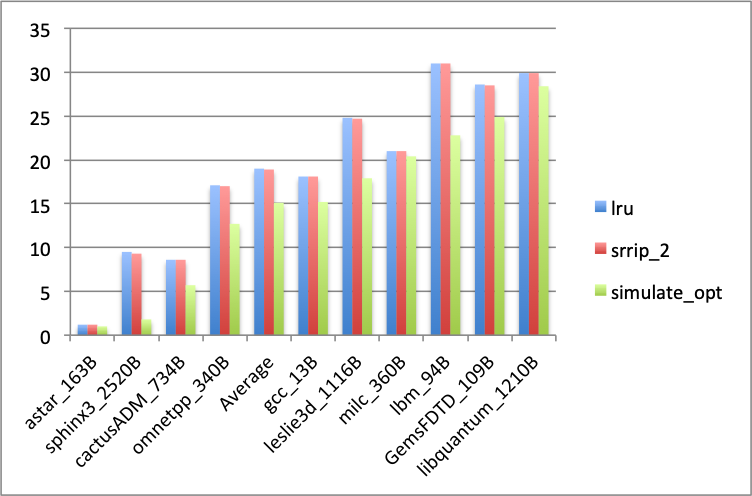
\includegraphics[height=.45\textheight]{distilled.png}
  \caption{LRU, SRRIP, and OPT policies only.}
\end{figure}

\begin{figure}[t]
  \centering
  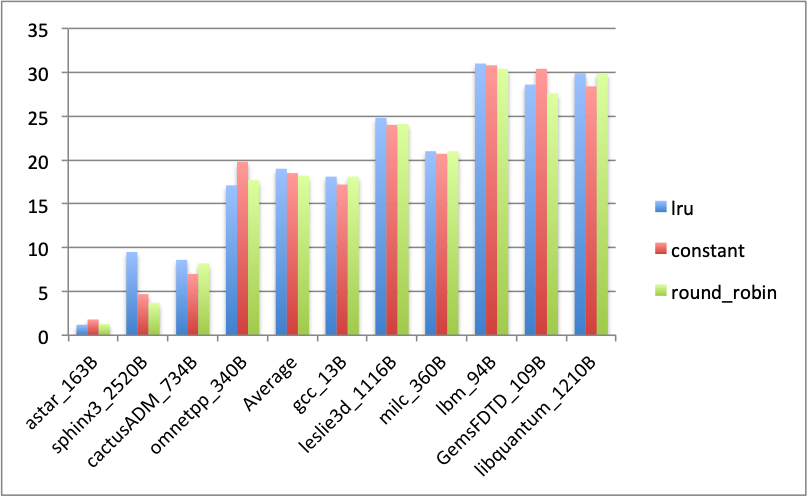
\includegraphics[height=.45\textheight]{round_robin_versus_constant.png}
  \caption{Round robin, constant, and LRU policies only.}
\end{figure}

\begin{figure}[t]
  \centering
  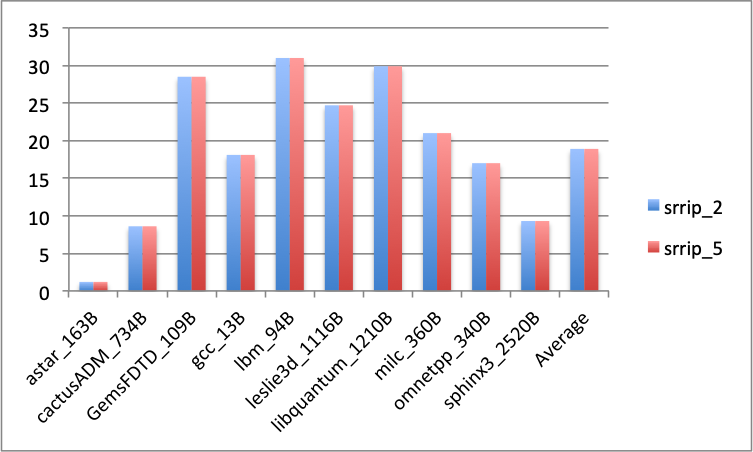
\includegraphics[height=.45\textheight]{ssrip_parameters.png}
  \caption{Static RRIP with $M = 2$ versus $M = 5$.}
\end{figure}

\begin{figure}[t]
  \centering
  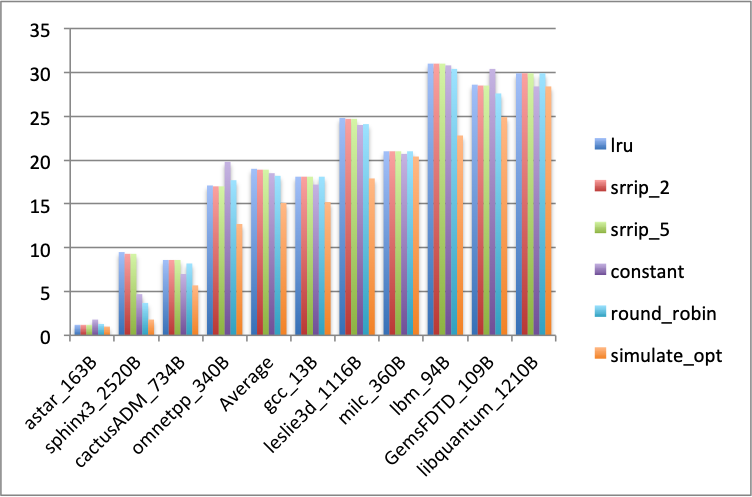
\includegraphics[height=.45\textheight]{everything.png}
  \caption{Side-by-side comparison of all experiments.}
\end{figure}


\end{document}